\chapter{AmoebaMCRT, modelling autofluorescence in skin for novel biomarkers of cardiovascular disease}
\label{chap:salvo}
\section{Introduction}

% motivation
% explain fluro method
% explain skin model
% explain nelder mead
% explain filter choice

% results in "2d" 
% results in 3d + higher
% future work


\section{Skin Model}

So far in this thesis all tissue models have been simplified, by assuming that tissue is a homogeneous structure with uniform optical properties.
However this is not the case in reality.
Tissue is very un-homogeneous, with non-uniform optical properties.
However to create a 1 to 1 model of tissue in a simulation is impractical due to the resolution required to resolve all the constituent part of the tissue down to the cell level.
Therefore we need to make a compromise between reality and what is possible to model efficiently.
To this end the section presents a 5 layer model of human skin. 
Dermatologists usually split the skin into 5 layers: Stratum Corneum, Epidermis\footnote{The epidermis can be split into several more layers, however these layers are optical similar and are rather small so we model just one layer here.}, Papillary Dermis, Reticular Dermis, and Hypodermis, see~\cref{fig:skinexample}.

\begin{figure}[!htpb]
    \centering
    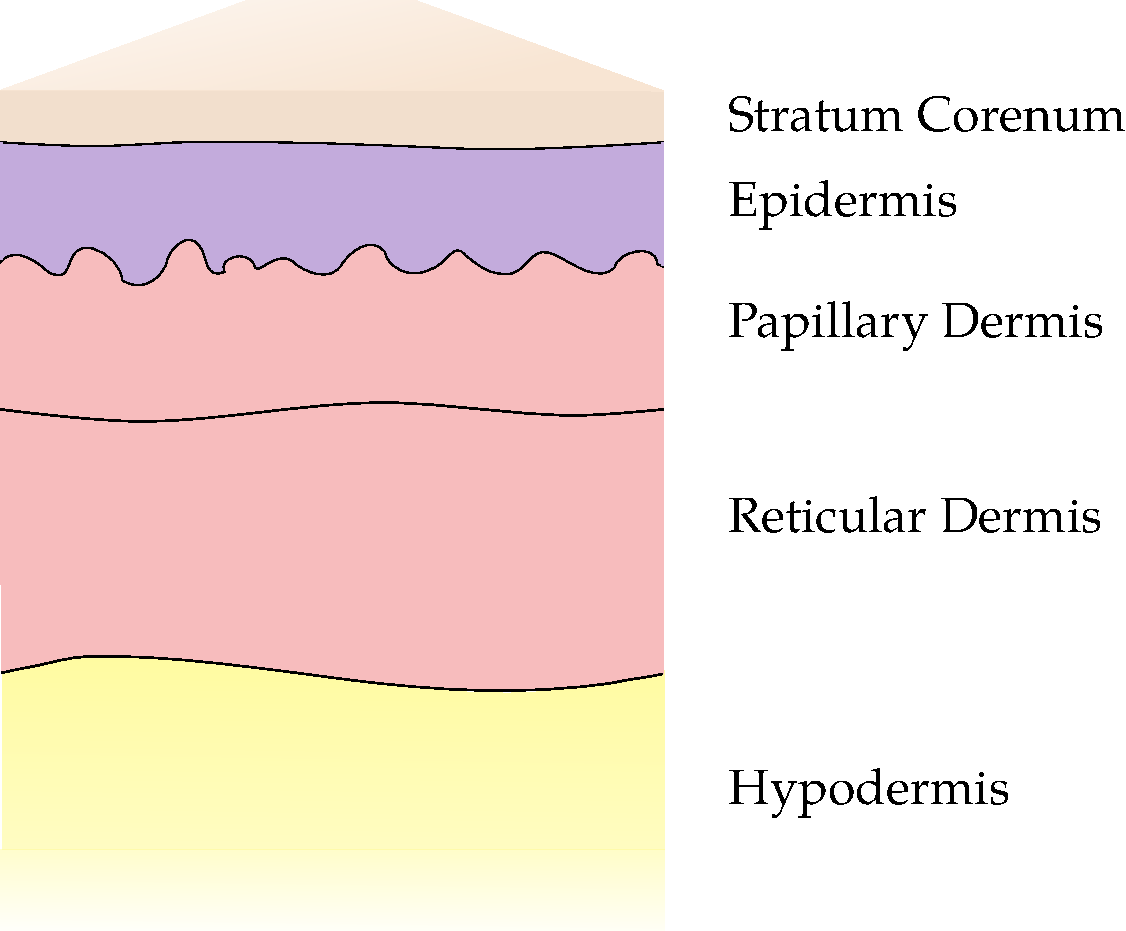
\includegraphics[width=0.7\textwidth]{Skin_layers.pdf}
    \caption{Illustration of skin layers in human skin.}
    \label{fig:skinexample}
\end{figure}

Each of these layers have various amounts of chromophores and scatterers.
To accurately model these various chromophores and scatterers, and therefore the skin, we must discuss the chemical makeup and spatial structure of the skin.

\subsection*{Stratum Corenum} % (fold)
\label{sub:stratum}

The top most layer of the skin is the stratum corenum.
This layer mostly consists of dead skin cells (keratinocytes).
The function of this layer is to be a protection barrier to prevent damage, infection and diffusion of unwanted chemicals.

% subsection stratum_corenum (end)

\subsubsection*{Epidermis} % (fold)
\label{ssub:epidermis}

Below the stratum corenum is the epidermis.
The epidermis consist of several layers that are optically similar so we restrict out model to modelling as one whole layer.
The layers that make up the epidermis are the stratum basale, stratum spinosum, stratum granulosum, and the stratum lucidum\footnote{The stratum corenum is usually part of the epidermis, however as its optical properties are different than that of the epidermis we model it as a separate layer.}.
The purpose of the epidermis is as before to provide a protective barrier to the underlying layers. 
The epidermis contains melanin which protects the stem cell keratinocyte which divide to form keratinocyte which form much of the upper layers of the skin.
In the stratum basale there is also melanocyte which produce the pigment melanin which is responsible for the color of the skin, and providing some protection from harmful UV light. 
Other types of cells found i the epidermis are Langerhans cells and Merkel cells which are part of the immune system and nervous system respectively.

% subsubsection epidermis (end)

\subsection*{Dermis} % (fold)
\label{sub:dermis}

The dermis is split into three different layers in our model: the papillary dermis, reticular dermis and the hypodermis.

The papillary dermis has blood

The reticular dermis has blood

The hypodermis consists of fat and  

% subsection dermis (end)

\subsubsection*{Optical Properties} % (fold)
\label{sub:optical_properties}

With a discussion of what makes up the skin, and what molecules contribute to the skins optical properties, this section gives an account of how our skin model, models the optical properties of skin.

To model blood, we first split blood into Deoxygenated and Oxygenated. We mix these two groups using the tissue oxygenation coefficient $S$. Blood absorption spectra are taken from%~\cite{}

\begin{equation}
\mu_{a,oxy/deoxy}=150\ \ln10\ \frac{\epsilon}{64458}
\label{eqn:oxy}
\end{equation}

\begin{equation}
\mu_{a,b}(\lambda) = SO_2\mu_{a,Oxy}+(1-SO_2)\mu_{a,DeOxy}
\label{eqn:blood}
\end{equation}

The next chromophores are bilirubin and $\beta$-carotene.
The absorption coefficients are calculated using the blah 

\begin{equation}
\mu_{a,Bilirubin}(\lambda)=\frac{\epsilon_{bilirubin}}{585}\ ln10\ C_{bilirubin}
\label{eqn:bili}
\end{equation}

\begin{equation}
\mu_{a,\beta-Caro}(\lambda)=\frac{\epsilon_{\beta-Caro}}{537}\ ln10\ C_{\beta-Caro}
\label{eqn:caro}
\end{equation}

To model melanin`'s absorption coefficient we use~\cref{eqn:eqn:melanin}, taken from...

\begin{equation}
\mu_{a,mel}(\lambda)=6.66\times10^{11} \times \lambda^{-3.33}
\label{eqn:eqn:melanin}
\end{equation}

Finally we use a base absorption coefficient to model the absorption due to the other parts of the skin that contribute to its optical properties, but individually do not have a large effect.

\begin{equation}
\mu_{a,b}=7.84\times10^{8}\times\lambda^{-3.255}
\label{eqn:base}
\end{equation}


\begin{figure}[!htpb]
	\centering
	% \includegraphics[width=0.75\textwidth]{}
	\caption{Absorption coefficients for the various chromophores found in skin.}
	\label{fig:absorcoeff}
\end{figure}





% subsubsection optical_properties (end)


\section{Modelling Fluorescence}

Fluroescene is the process in which light of a certain wavelength is incident on a molecule, the molecule absorbs the light and re-emits the light at a new longer wavelength.

\Cref{fig:Jabo} shows an example of Jablonski diagram.

\begin{figure}[!htpb]
	\centering
	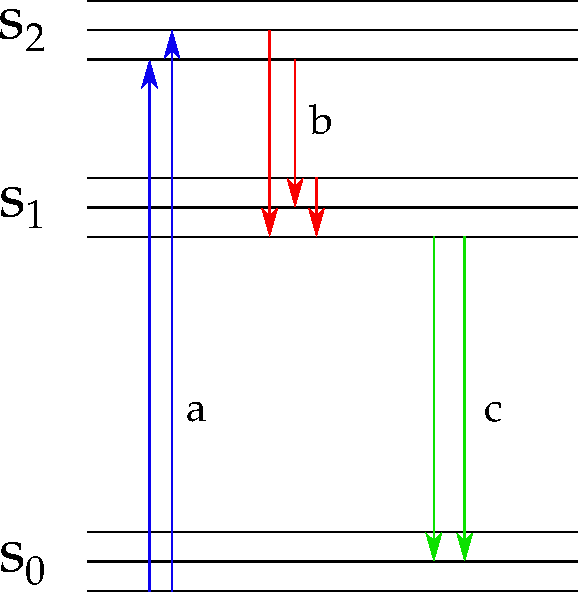
\includegraphics[width=0.45\textwidth]{jabo-diag.pdf}
	\caption{Jablonski diagram for PPIX. a) excitation of the ground state via absorption of a photon, b) non-radiative transition, and c) fluorescence.}
	\label{fig:Jabo}
\end{figure}

To model fluorescence from multiple fluorophores requires a change of the \gls*{mcrt} code presented thus far.
This change is to the interaction portion of the algorithm, so that it will now include the option for a packet to undergo fluorescence.
To calculate whether a packet absorbs, scatters or fluoresces, first the probability of each of these events must be calculated.
Discussion of scattering and absorption (by the bulk medium) was described in~\cref{sec:opticalprops}.
To calculate the probability of fluorescence, we first assume that the quantum yield of the molecule is unity.
This is physically unrealistic, however it does not affect the simulations accuracy, as modelling a realistic quantum yield would mean that more packets would be discarded, and thus the signal to noise ration would be worse than if we assume a quantum yield of unity.
To calculate the probability of fluorescence, the absorption coefficient of the florescent molecule must be calculated.
This is shown in~\cref{eqn:flurodef}:

\begin{equation}
\mu_f=\ln\left(10\right) C \varepsilon
\label{eqn:flurodef}
\end{equation}

Where $C$ is the concentration of the fluorophore, $\varepsilon$ is the extinction coefficient of the fluorophore, and $ln(10)$ is the natural logarithm of 10\footnote{This factor appears as historically $\varepsilon$ was measured in base 10~\cite{jacques2013optical}.}.\\

The next step is to calculate the total attenuation coefficient for a given species as in~\cref{eqn:totdef}

\begin{equation}
\mu_{t_i}=\mu_{s_i}+\mu_{a_i}+\mu_{f_i}
\label{eqn:totdef}
\end{equation}

Where as usual $\mu_a$ and $\mu_s$ are the absorption and scattering coefficients, and $\mu_f$ is the fluorescence coefficient as defined in~\cref{eqn:flurodef}.
As the absorption coefficient of fluorophores are small in comparison to the medium, and that the absorption coefficient of fluorescent molecules are generally much larger than that of their scattering coefficient, we assume that the scattering coefficient is negligible.
Finally we calculate the probability of interacting with a given species using~\cref{eqn:totspec}

\begin{equation}
P_i=\frac{\mu_{t,i}}{\sum\limits_{i=1}^{N} \mu_{t,i}}
\label{eqn:totspec}
\end{equation}

Where $P_i$ is the probability of interacting with the $i^{th}$ species, the numerator is the attenuation coefficient for $i^{th}$ species, and the denominator is the total attenuation coefficient for all the species.

\cref{algo:speciespick} shows the process used to determine which species to interact with.

\newpage

\begin{center}
\begin{algorithm}[H]
\SetAlgoLined
  set $\mu_{tot}$\;
  set all $P_i$'s\;
  set $\xi_1$\;
  \uIf{$\xi_1 < P_1$}{
    set $\xi_2$\;
    \uIf{$\xi_2 < a_m$}{
      Scatter in medium\;
     }
     \Else{
      Absorb in medium\;
     }
  }
  \uElseIf{$\xi_1 < P_1 + P_2$}{
    Species 1 fluoresces\;
  }
  \uElseIf{$\xi_1 < P_1 + P_2 + P_3$}{
    Species 2 fluoresces\;
  }
  \uElseIf{$\xi_1 < P_1 + P_2 + P_3 + ... + P_n$}{
    Species n fluoresces\;
  }
  \Else{
    Error\;
  }
\
\caption{\textit{An algorithm to determine which species to interact with. $P_1$ is the probability of interacting with the bulk medium, $P_2$ to $P_n$ is the probability of interacting with a fluorescent species, $a_m$ is the albedo of the bulk medium, $\xi_i$ is a random number, and $\mu_{tot}$ is the total attenuation coefficient of all the species summed.}}
\label{algo:speciespick}
\end{algorithm}
\end{center}

This method allows an arbitrary number of fluorophores to be modelled.


\section{Nelder-Mead Method}

The \gls*{nm} method is an algorithm for unconstrained optimisation. 
The algorithm is based upon iteratively updating a simplex. 
A simplex is a structure in $n-dimensional$ space, consisting of $n+1$ points that are not in the same plane. 
Therefore in 1D, the simplex is a line, in 2D a triangle, in 3D a tetrahedron, etc.. 
The Nelder-Mead method is a gradient free method, meaning that it does not require derivative to be calculated and that the search space does not need to be smooth.

The algorithm works by removing the worst vertex of the simplex and replacing it with a `better' vertex calculated via a number of different operations.
These operations can be seen in~\cref{fig:NM-operations}.

The first step of the~\gls*{nm} method is to sort the initial vertices according to their fitness.
For $n=2$, we define $x_w$ as the `worst' point, $x_l$ and the `lousy' point, and $x_b$ the `best' point, such that $f(x_b)\leq f(x_l)\leq f(x_w)$, where $f(x)$ is evaluating the `fitness' of a point $x$.
With the vertices sorted, the centroid of the simplex is calculated as in~\cref{eqn:centroid}.
The centroid is the mean of all the vertices bar the `worst' point.

\begin{figure}[!htbp]
    \centering
    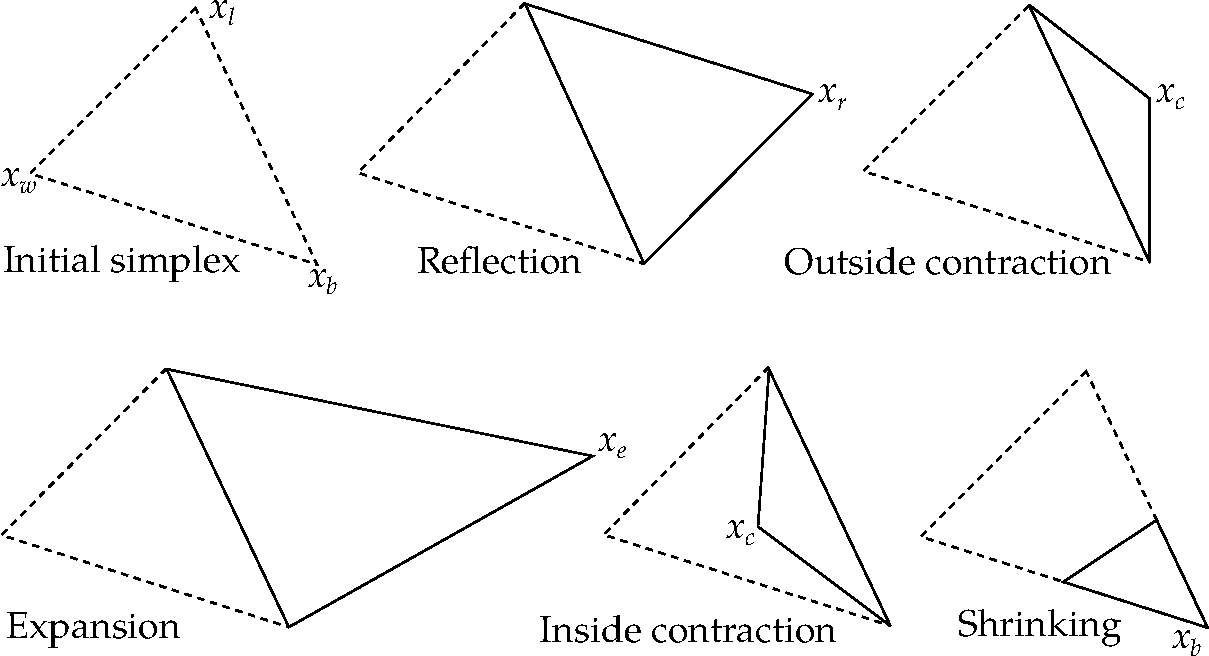
\includegraphics[width=0.75\textwidth]{simplex-operations.pdf}
    \caption{Operations that can be preformed on a simplex for $n=2$.}
    \label{fig:NM-operations}
\end{figure}

The next step is to move the simplex via a reflection.
To calculate the new vertex via reflection~\cref{eqn:reflect} is used, where $\alpha$ is the reflection factor.
If this new point, $x_r$, is better\footnote{Here better means the point has a lower fitness score, as we use $\chi^2$ metric to assess the fitness of a point.} than the current `best' point then we calculate a new point in the same direction but further using the expansion operation~\cref{eqn:expand}, where $\gamma$ is the expansion factor.
If this new point, $x_e$, is better than the `best' point then we replace $x_w$ with $x_e$ and start the process again.
However is $x_e$ is not better than the `best' point, then we discard it and replace the worst point with $x_r$ the reflected point.

If when calculating $x_r$, we find that is worse than the `best' point, we then check if $x_r$ is better than the `lousy' point.
If $x_r$ is better than $x_l$ then we replace the `worst' point and start the process again.
However if the $x_r$ is worse than $x_l$, we then compare it to the `worst' point.
If $x_r$ is better than the `worst' point then we preform and inside contraction~\cref{eqn:insidecontract}, where $\beta$ is the contraction factor.
If this new point, $x_{ic}$, is better than the `worst' point then we keep it, otherwise we preform the shrink operation, shrinking the whole simplex around the `best' point.

If $x_r$ is not worse than the `worst' point then we preform an outside contraction~\cref{eqn:outsidecontract}.
This computes a new point $x_{oc}$.
If $x_{oc}$ is better than $x_w$, then we keep it, otherwise again we shrink around the `best' point.

The process described above is summarised in~\cref{fig:NM-algo}.
Standard values for the factors are: $\alpha=1$, $\beta=\frac{1}{2}$, and $\gamma=2$.
Though in practise these values are adjusted for the problem at hand.

\begin{align}
c &= \frac{1}{n}\sum \limits_{i=1,i\neq w}^{n+1} x_i \label{eqn:centroid}\\
x_r &= c + \alpha(c - x_w)\label{eqn:reflect}\\
x_e &= c + \gamma(x_r - c)\label{eqn:expand}\\
x_{oc} &= c + \beta(x_r - c)\label{eqn:outsidecontract}\\
x_{ic} &= c + \beta(x_w - c)\label{eqn:insidecontract}
\end{align}

As the Nelder-Mead method has no inbuilt convergence criteria, this must be added.
We use two different criteria based upon simplex size, and vertex fitness.
The criteria for the simplex size is as; if the size of the simplex(~\cref{eqn:sizeof})
Where $p_i$ and $p_{i+1}$ are vertices in the simplex that are connected by and edge. 

\begin{equation}
size=\sum\limits_{i=1}^{n+1}|p_{i}-p_{i+1}|
\label{eqn:sizeof}
\end{equation}

If the size of the simplex falls below a pre-set value, then we preform a factorial test to see if the simplex should be restarted or if the algorithm should terminate.
The factorial test checks the space around the current simplex to ensure that we have converged to a global minima.
If the check fails then the algorithm is restarted with the current best point kept, and new vertices generated.

\begin{figure}[!htbp]
    \centering
    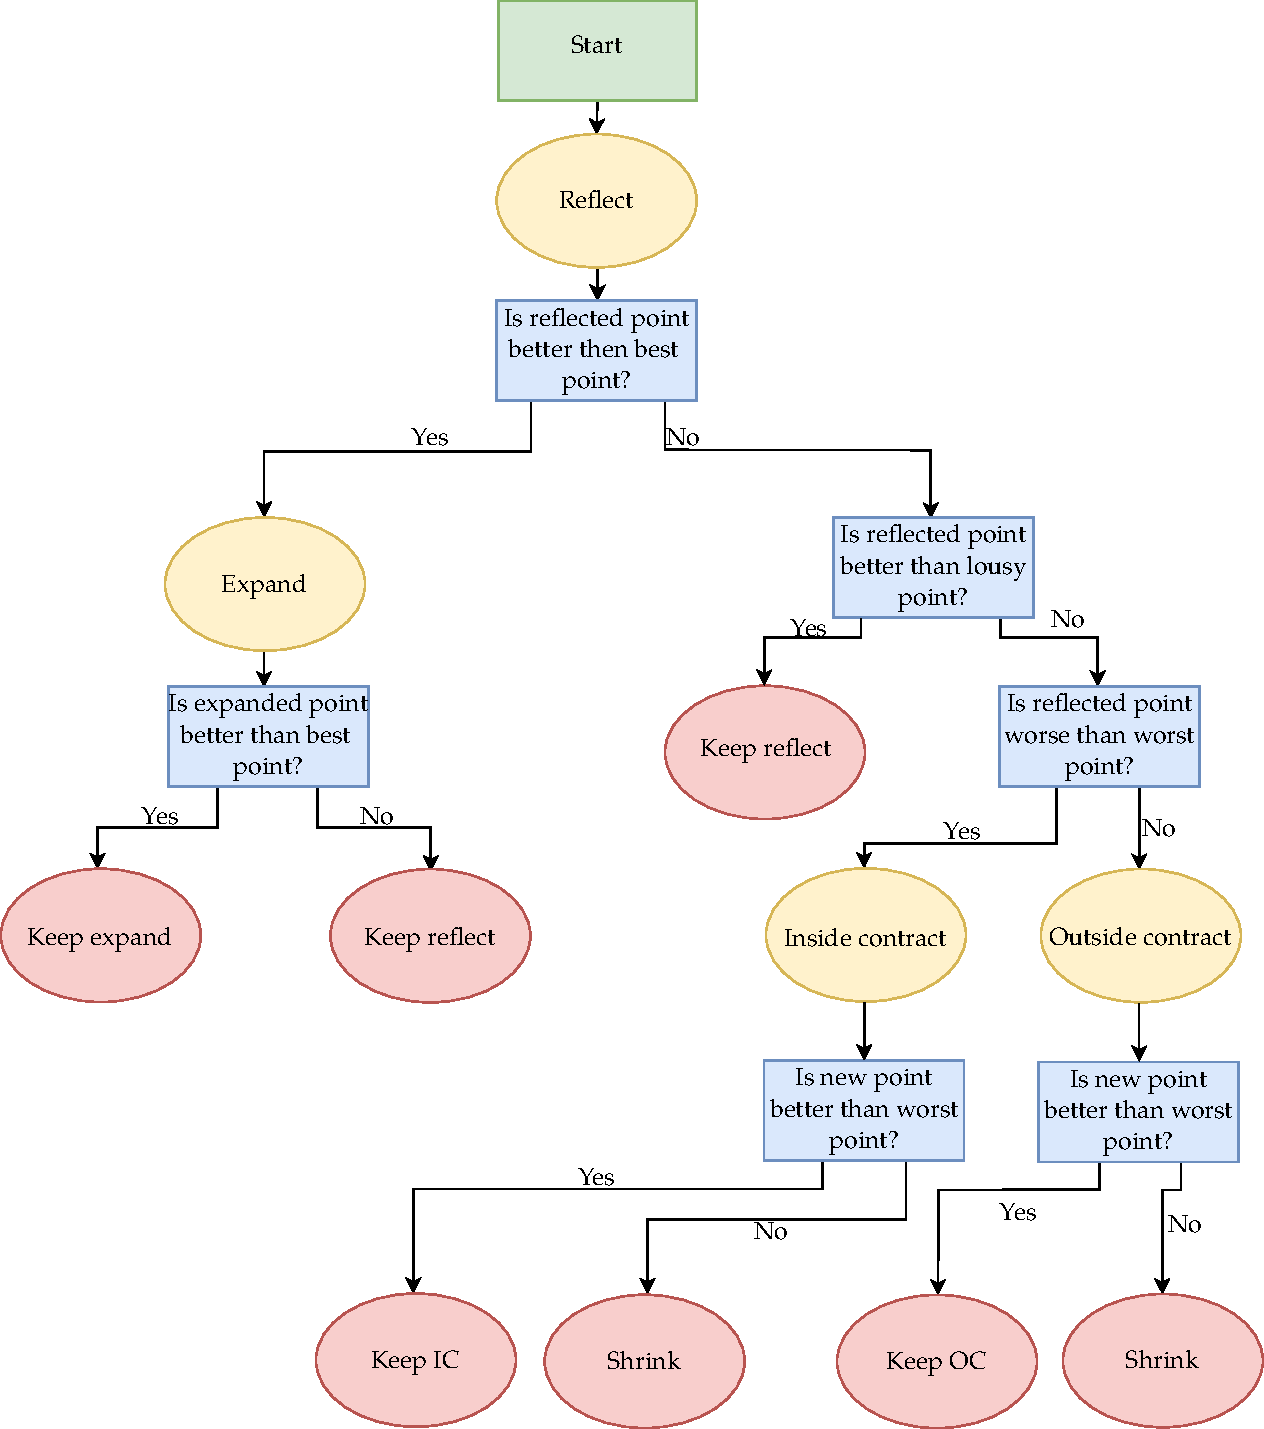
\includegraphics[width=0.65\textwidth]{flowchart.pdf}
    \caption{Nelder-Mead decision tree}
    \label{fig:NM-algo}
\end{figure}

The other convergence criteria is the a check to see if the best point is `good enough'.
The current best point is compared to a pre-set fitness value.
If the best point is better than the pre-set value then the algorithm terminates.

\FloatBarrier
\section{Validation}
The~\gls*{nm} method was coded in Fortran, so that it could be easily interfaced with the~\gls*{mcrt} code developed as part of this thesis.
To test that the method works as intended a number of trial functions were tested, see~\cref{tab:testfuncs}.
This was achieved by selecting an initial simplex, and the method allowed to iterate until it converged.
The results of this are shown in~\cref{fig:nmtest}.


\begin{table}[]
    \begin{tabular}{|c|c|c|}
    \hline
        Name         & Formula                                                                & Global Minumum                \\ \hline
        Sphere       & $x^2+y^2$                                                              & $f(0,0)=0.$                   \\ \hline
        Rosenbrock   & $(a-x)^2+b(y-x^2)^2$                                                   & $f(1,1)=0.$                   \\ \hline
        Ackely       & $ -20\exp\left[-0.2\sqrt{0.5\left(x^{2}+y^{2}\right)}\right] - $       & $f(0,0)=0.$                   \\
                     & $\exp\left[0.5\left(\cos 2\pi x + \cos 2\pi y \right)\right] + e + 20$ &                               \\ \hline
        Himmelblau's & $(x^2+y-11)^2+(x+y^2-7)^2$                                             & $f(3,2)=0., $                 \\
                     &                                                                        & $f(-2.805118,3.131312)=0.,$   \\
                     &                                                                        & $f(-3.779310,-3.283186)=0.,$  \\  
                     &                                                                        & $f(3.584428,-1.848126)=0.$    \\ \hline
    \end{tabular}
    \caption{Table of standard test functions for numerical optimisation.}
    \label{tab:testfuncs}
\end{table}


\begin{figure}[!htbp]
    \centering
    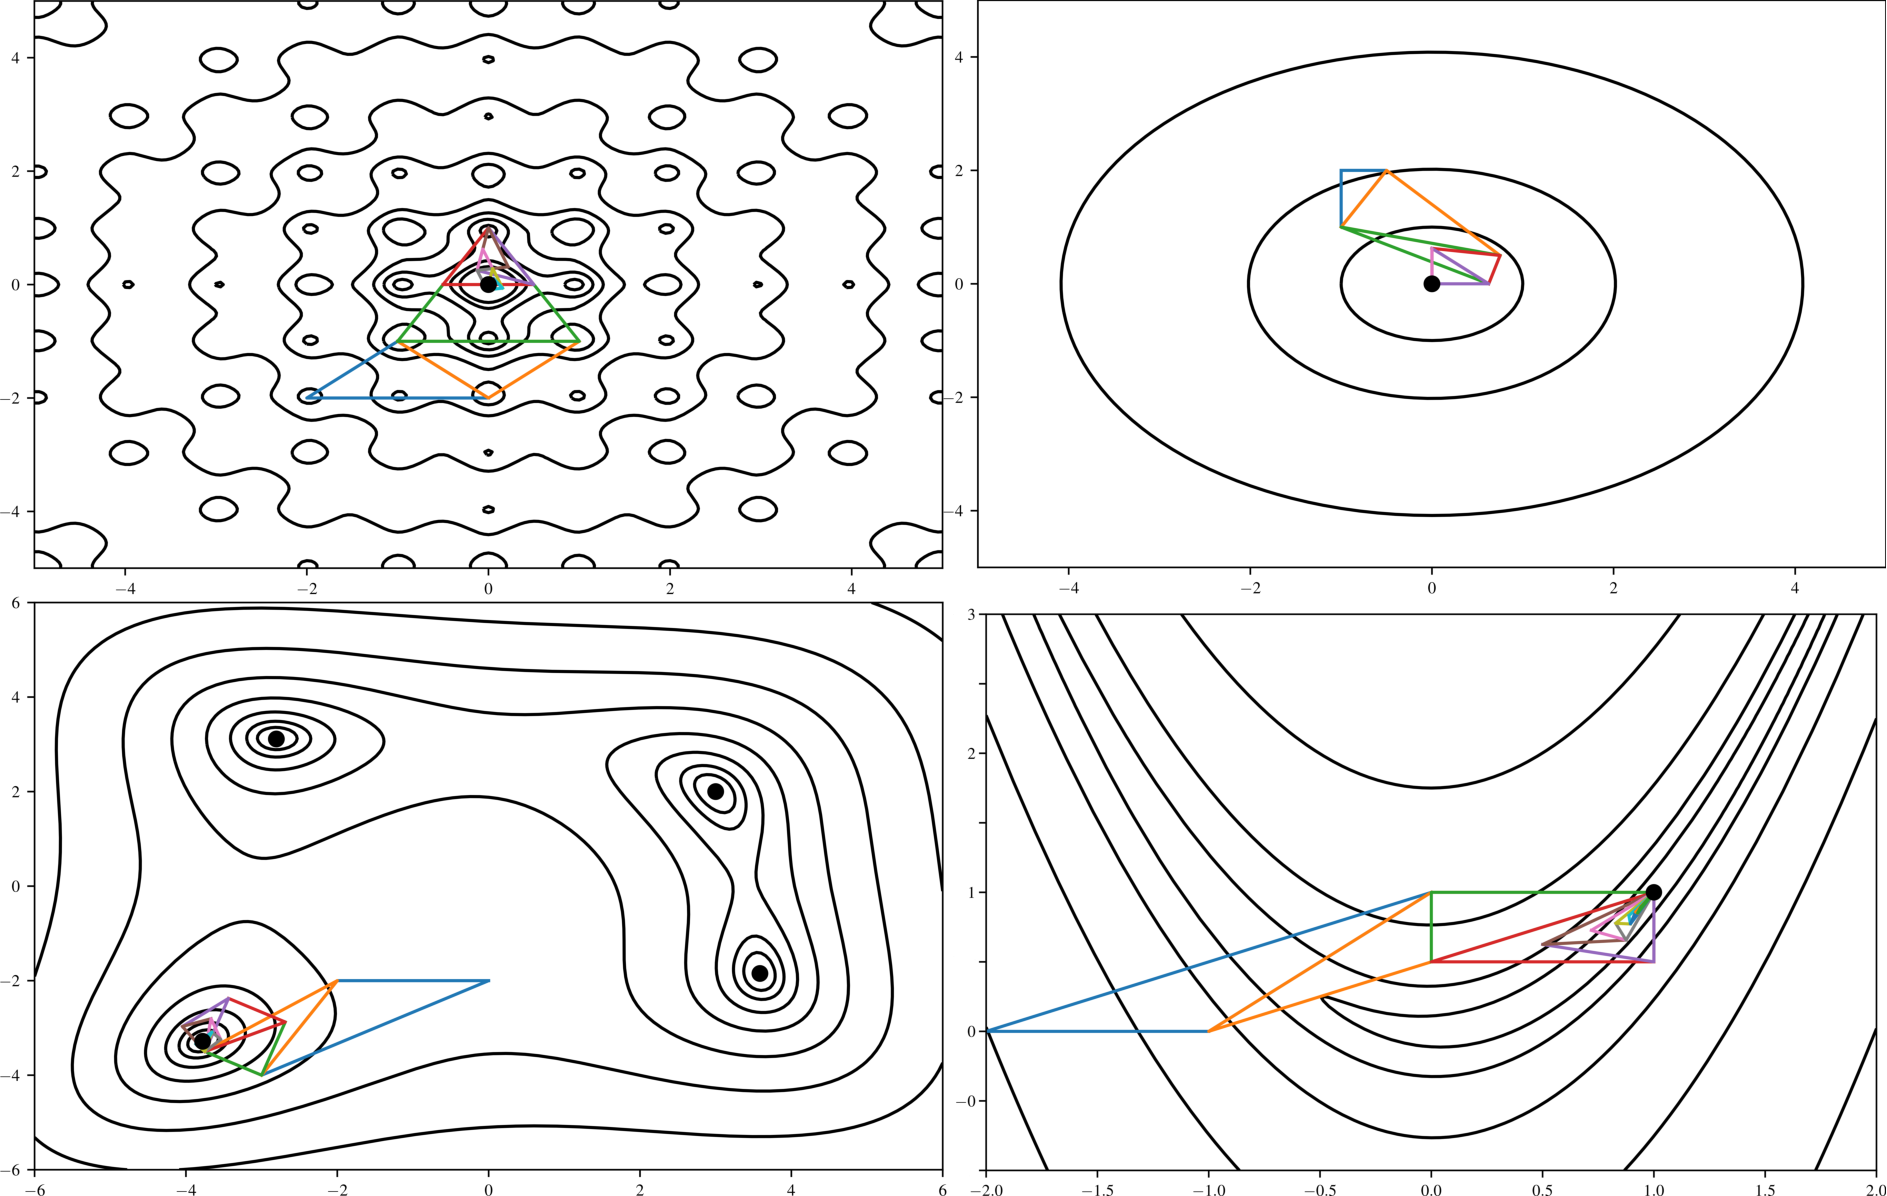
\includegraphics[width=0.75\textwidth]{all-nm-tests.pdf}
    \caption{Contour plots of test functions with Nelder-Mead simplexes over plotted. Top left is the Ackely function, top right is the sphere function, bottom left is the Himmelblau's function, and the bottom right is the Rosenbrock function. Blue simplex is the initial simplex, and the large black dots represent the Global minima.}
    \label{fig:nmtest}
\end{figure}

To ensure that the~\gls*{nm} method can be used to find the unknown concentrations of the autoflurophores, we test the method with a known model.
This model consists of three different fluorophores: NADH (nicotinamide adenine dinucleotide), FAD (flavin adenine dinucleotide), and a fictitious fluorophore that has similar properties to NADH and tyrosine, such that the excitation spectrum is that of NADH and the emission spectrum is that of tyrosine.
The three fluorophores are distributed in the stratum corenum (NADH), epidermis (FAD), and the papillary dermis (fictitious).
The concentration in these layers is such that the bulk optical properties are not affected: NADH has a concentration of $x$, FAD $y$, and the fictitious fluorophore has a concentration of $z$.

As many models need to be run in order to determine whether a global maxima has been reached using the NM method and the fluorophore concentration low many packets need to be run.
Therefore the ~\gls*{mcrt} algorithm has to be computationally efficient in order to arrive at an answer within a reasonable time.
To this end the 3D skin model is shrunk to a 1D model so that the optical integration routine can efficiently move the photon through the simulated medium.
The optical properties of the incident wavelength are also stored so that when a new photon is started the optical properties can easily be adjusted without need for any calculation.


\begin{figure}[!htbp]
	\centering
	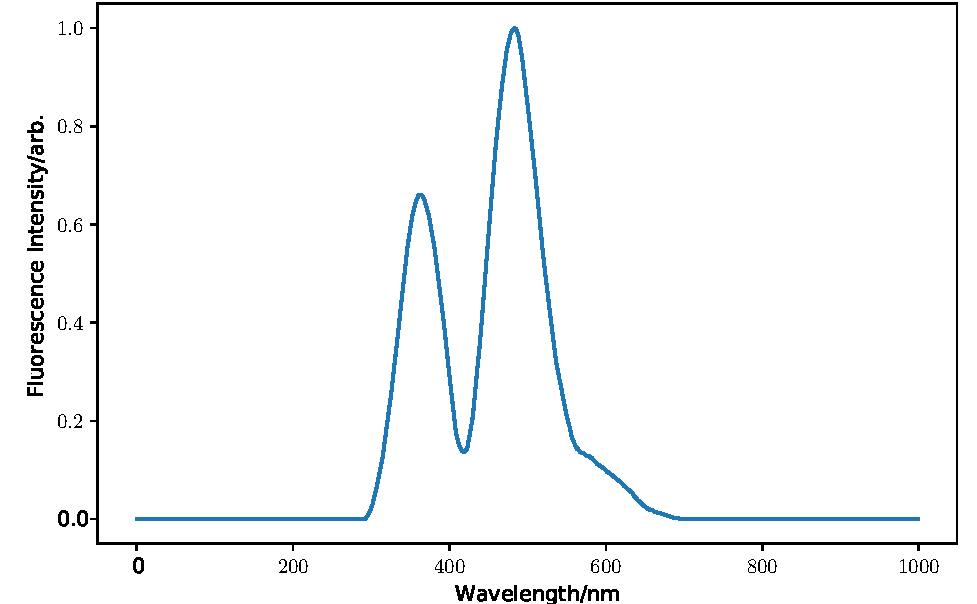
\includegraphics[width=0.6\textwidth]{target-toy.pdf}
	\caption{Example of toy model for testing NM method. The three peaks correspond to the fictitious fluorophore, NADH, and FAD respectively.}
	\label{fig:figure1}
\end{figure}

We first run this model through the MCRT to get an output spectrum.
We then test the~\gls*{nm} method for $n=2$ and $n=3$.

\section{Results}

\begin{figure}[!htpb]
    \centering
    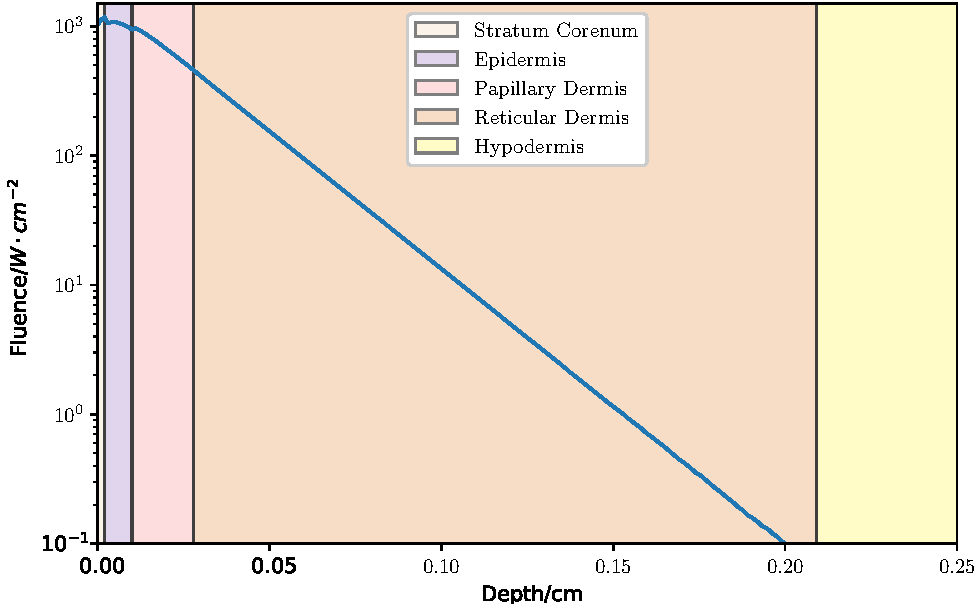
\includegraphics[width=0.75\textwidth]{UV-fluence-365nm.pdf}
    \caption{Penetration of UV radiation as a function of depth.}
    \label{fig:uvpen}
\end{figure}

\section{Discussion}
\section{Conclusion}

We have presented out code, AmoebaMCRT, which combines the Nelder-Mead method and MCRT in order to determine the concentrations of naturally occurring fluorophores in human skin.


%AF Code works, tested against toy model, may need further validation. 

%No paper or aim for project. Need contact with Dundee/Ninewells to proceed.
